\documentclass[a4paper]{article} %style de document
\usepackage[utf8]{inputenc} %encodage des caractères
\usepackage[french]{babel} %paquet de langue français
\usepackage[T1]{fontenc} %encodage de la police
\usepackage[top=2cm,bottom=2cm,left=2cm,right=2cm]{geometry} %marges
\usepackage{graphicx} %affichage des images
\usepackage{hyperref}%rend actif liens et références
\usepackage{verbatim}%permet insertion de texte brut (du style le logo Latex)
%\usepackage{amssymb} %collection de symboles
\usepackage[dvipsnames]{xcolor}%importe les couleurs, l'option permet d'avoir encore plus de couleurs
\usepackage{sectsty}%permet de changer les couleurs des sections/titres, etc
\usepackage{tikz}%pour faire des figures
\definecolor{astral}{RGB}{46,116,181}
\sectionfont{\color{red}}
\subsectionfont{\color{Blue}}
\subsubsectionfont{\color{NavyBlue}}
\usepackage{appendix} % Pour l'annexe

\title{\vspace*{5cm}
\LARGE{\em{Rapport Conception logicielle avancée}}\\
Solveur de Ricochet Robots\\\vspace*{0.5cm}
UE Conception de Logiciels\\
Licence Informatique
}
\author{
Elie Malbec - Alex Lefevre -  Yoann Kablan - Vouvou Brandon\\
Groupe 1B
}

\date{2019 - 2020}

\begin{document}
\maketitle
\newpage
\tableofcontents
\newpage

\section{Introduction}
Dans le cadre de l'unité d'enseignement Conception Logicielle Avancée, nous avons formé un groupe de quatre étudiants : Alex Lefevre, Elie Malbec, Yoann Kablan, Brandon Vouvou pour créer un solveur de Ricochet Robots.

Le choix du sujet s'est fait naturellement, le concept du jeu et la réalisation d'un solveur nous ont motivés.

Le langage de programmation imposé est le Java.

\section{Description du jeu et des objectifs}
	\subsection{Le jeu Ricochet Robot}
Ricochet Robot est un jeu de plateau carré composé de pions robots et de tuiles objectifs. Le but est de trouver la séquence de mouvements nécessaires pour emmener le robot principal sur un objectif. Cependant, chaque déplacement ne peut se faire qu'en ligne droite jusqu'au prochain obstacle. Chaque case du plateau peut comporter des murs faisant office d'obstacle.

Une partie démarre par le tirage au sort d'une cible parmi les dix-sept présentes sur le plateau. Un robot est également tiré, il devra se rendre sur cet objectif pour terminer le jeu.

Il est possible de déplacer les trois autres robots pour arriver à la destination. Le but du jeu est de résoudre ce puzzle avec le moins de mouvements possible dans un temps limité. C'est également le but de notre projet.

	\subsection{Objectif du solveur}
L'objectif de la résolution du jeu est de minimiser le nombre de déplacements nécessaires pour permettre au robot principal de se rendre sur l'objectif. Plusieurs solutions permettent d'arriver au résultat mais certaines sont plus rapides.

Nous avons ainsi développer une algorithme résolvant le puzzle et minimisant le nombre de coups suivant une complexité de calcul donnée. Toute situation de jeu permet de trouver une solution au problème.

\section{Développement du moteur de jeu}
	\subsection{Modèle physique}
		\subsubsection{Le plateau de jeu}
Le modèle physique du jeu repose sur un plateau découpé en 256 cases reparties sur 16 lignes et 16 colonnes. Ces cases comportent à la fois des murs qui bloquent les mouvements et des entités.
Les murs sont situés dans les quatre directions cardinales et délimitent à la fois la terrain de jeu avec une bordure extérieure et forment des angles entre eux pour y placer les objectifs.
Il y a quatre robots et dix-sept objectifs (cibles) sur la version officielle.

Le terrain de jeu est en réalité découpé en quatre sous terrains de 8 lignes et 8 colonnes. Le placement de ces derniers et leur rotation apporte de nombreuses configurations de jeu, mais toujours solvables.

Pour notre projet, nous nous sommes tenus de respecter la configuration du jeu officiel en utilisant quatre robots et dix-sept objectifs. Le plateau de jeu est quand à lui soit chargé depuis le plateau officiel, soit généré aléatoirement.

		\subsubsection{Déplacements internes}
Les déplacements des robots sur le plateau doivent suivre les quatre directions cardinales : Nord, Sud, Est et Ouest. Un robot ne peut se déplacer dans la case adjacente uniquement si aucun mur ne bloque le déplacement sur sa position mais également qu'aucun robot n'est présent sur la case adjacente.

Un objectif sur une case ne constitue pas un obstacle pour un déplacement.

Notons que bouger un robot permet de créer un nouvel obstacle à une certaine position du jeu pouvant aider à la résolution. À chaque robot déplacé, un mouvement supplémentaire est comptabilisé.

	\subsection{Modèle informatique}
		\subsubsection{Plateau du jeu}
Pour le modèle informatique du plateau, nous avons développé une classe \texttt{Board}. Cette dernière est constituée de 256 cases et représente l'état actuel du jeu. Les entités sont représentées par des classes \texttt{Robot} et \texttt{Goal}. Chaque robot ou cible ne sont pas directement placés dans une case mais ils possèdent leur position sur le plateau de jeu sous forme de coordonnées $x$ et $y$.
Les coordonnées dans le plateau suivent le graphique \ref{coordPlateau}.

\begin{figure}[!h]
	\begin{center}
	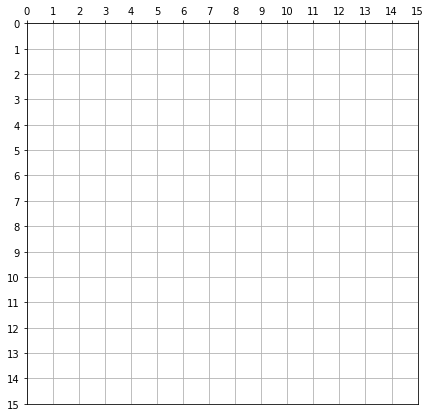
\includegraphics[scale=0.5]{./images/board.png}
	\caption{Plateau de jeu sous forme de coordonnées}\label{coordPlateau}
	\end{center}
\end{figure}

Les robots et les objectifs (cibles) sont stockées dans des listes avec la structure \texttt{ArrayList}. Des références au robot principal et à la cible principale permettent de les distinguer des autres.

La construction du plateau de jeu est basée sur un fichier texte, il donne pour chaque coordonnée les murs et entités présentes (cf:\ref{structFichier}). Cette construction est par défaut basée sur celle du plateau de jeu officiel. Mais il est possible de générer un plateau aléatoirement ou de choisir un fichier de configuration.

Voici le diagramme de classe donnant les principales méthodes utilisées sur le plateau mais également la structure des robots et cibles.

\begin{figure}[!h]
	\begin{center}
	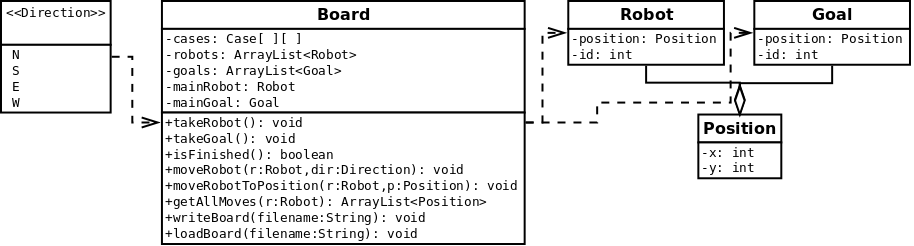
\includegraphics[scale=0.5]{./images/boardwithentities.png}
	\caption{Diagramme de classe du Board et des entités}
	\end{center}
\end{figure}

Le plateau dispose de méthodes qui lui permettent de bouger les robots, de tester si le jeu est terminé mais aussi de tirer une nouvelle cible ou un nouveau robot. Les directions sont listées depuis une énumération et les positions représentés avec deux coordonnées pour un plan deux dimensions.

Nous pouvons également remarquer que les 256 cases sont des objets \texttt{Case} stockées dans un double tableau. Cela permet un accès direct aux données mais aussi un parcours simplifié avec une largeur et une hauteur connue. La composition d'une case est la suivante :
\begin{figure}[htpb]
	\begin{center}
	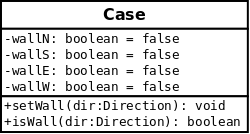
\includegraphics[scale=0.5]{./images/casediag.png}
	\caption{Classe Case}
	\end{center}
\end{figure}

Les quatre murs possibles sont par défaut désactivés puis activés avec la méthode \texttt{setWall} dans la direction donnée. Une fois les murs mis en place, ils ne changent plus durant la partie.

		\subsubsection{Déplacements internes}
Concernant les déplacements, les méthodes \texttt{moveRobot} et \texttt{getAllMoves} requiert des tests supplémentaires. Il faut vérifier que les déplacement sont valides et donner les position d'arrivée quand un obstacle est rencontré. Pour cela, des méthodes ont été implémentées dans la classe \texttt{Board} dont voici le diagramme :

\begin{figure}[htpb]
	\begin{center}
	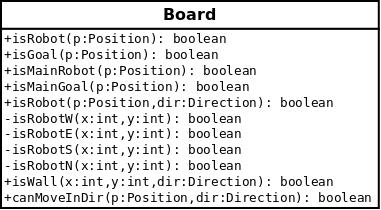
\includegraphics[scale=0.5]{./images/boardMove.png}
	\caption{Méthodes pour déplacements dans Board}
	\end{center}
\end{figure}

Les déplacements sont ainsi possibles en donnant un robot et une direction à la méthode \texttt{moveRobot} et le déplacement est effectué. C'est à dire que la position d'arrivée est déterminée suivant la direction puis le robot concerné voit sa position modifiée.

	\subsection{Visualisation d'un plateau de jeu}
Pour permettre les tests et rendre le jeu plus visuel, une interface graphique à été développée en suivant le modèle Modèle Vue Contrôleur. Les murs sont représentés par des traits et les entités sont placées par rapport à leurs coordonnées respectives. Le robot principal est coloré en rouge et la cible principale en vert. Cette visualisation permet de mieux voir les données comparativement à une lecture descriptive sous forme textuelle.
La figure \ref{visuBoard} donne un aperçu de la vue sur le \texttt{Board}.

\begin{figure}[htpb]
	\begin{center}
	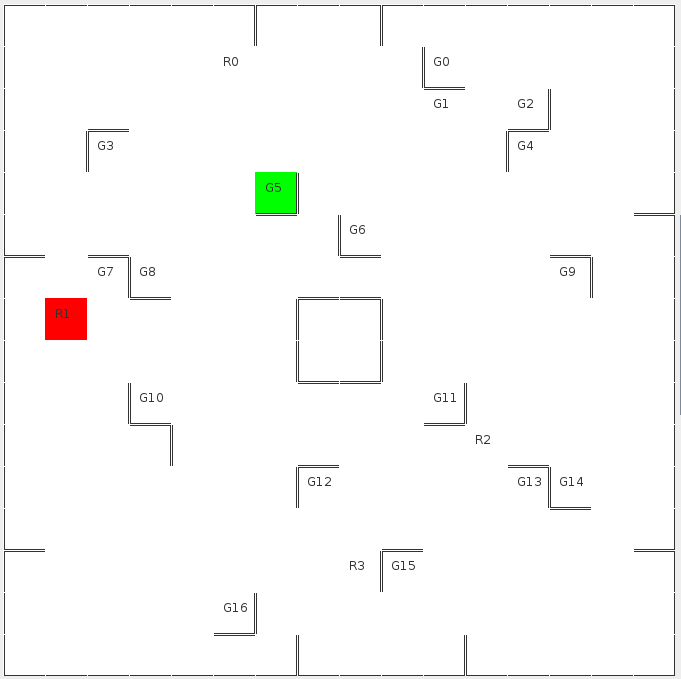
\includegraphics[scale=0.4]{./images/visuBoard.png}
	\caption{Visualisation graphique du jeu}\label{visuBoard}
	\end{center}
\end{figure}


\section{Fonctionnalités implémentées}

\subsection{DESCRIPTION  DES FONCTIONNALITÉS }
Au cours du projet , de multiples fonctionnalités ont été implémentées...Pour commencer nous avons implémenté le jeu et sa structure c'est-à-dire le plateau et tous les éléments qui le constitue ce plateau sont un plateau de n*m objets de types cases qui ont comme attribut quatre booléens qui sont ici nos murs. Ce plateau est constitué de plusieurs éléments c'est-à-dire les murs qui sont placés de façon aléatoire ou chargé à partir d’un fichier ces murs sont comme toute logique non traversable et formant souvent des angles qui contiennent souvent ou pas des cibles . Ensuite nous avons implémenté les différentes entités du jeu : les robots qui sont dotés de plusieurs attributs dont la position  et l’identifiant ils ont aussi la possibilité de se déplacer en ligne droite uniquement  ensuite les cibles qui ont les mêmes attributs que les robots qui sont entre autres la position et l’identifiant ainsi dans le plateau de jeu une de ses cibles est considéré comme  l'objectif principal . Nous avons accompagné cela d’une interface graphique là où il est possible d'afficher le plateau présent dans la console, enregistrer le plateau  ensuite  d’exécuter l’algorithme A* et enfin de remettre à zéro le plateau. Notre jeu ne se joue pas en console bien qu’il soit possible d’afficher le plateau de jeu avec des robots et même des déplacements dans la console.puis enfin de l’algorithme de résolution A* qui partant de la position de départ d’un robot trouve les positions intermédiaires jusqu’à la résolution du jeu . 


		\subsubsection{ ORGANISATION DU PROJET 
}
L'organisation du projet s'est déroulée en plusieurs étapes importantes, la première concerne la structure du projet. Les premières séances ont été consacrées au choix du projet. Après cela fallait commencer par coder le plateau et les éléments qui le constituent Bien avant d’avoir commencé à coder ensemble le jeu  Élie avait déjà une implémentation du plateau de jeu, ainsi Lors de la deuxième séance de Travaux pratiques  nous avons commencé à coder le plateau et les éléments qui le constituent c'est-à-dire les murs et les autres entités nous créons alors la première version de notre  jeu ricochets robot qui était la version robot 1.1 travail qui fut validé par tous les membres du groupe.Par la suite Alex a avancé sur la structuration du plateau  pendant que Yoann et Élie  commençaient à implémenter les déplacements des robots et les possibilités de déplacements des robots dans le plateau . Après plusieurs implémentions et test nous avons réuni nos idées pour finaliser cela. Une première version du projet était fonctionnelle en console et permettait déjà de :  choisir la cible principale de façon aléatoire, de sélectionner le robot principal, d’effectuer des déplacements, de charger un plateau prédéfini, de générer un plateau avec des constituants placés aléatoirement tout en respectant les normes du jeu.Après cette phase, Nous nous sommes directement penchés sur l’interface graphique partie où les connaissances d’Alex nous ont beaucoup aidés. À partir de ce moment , le projet s’est scindé en deux parties : Alex travaillait sur l’interface pendant que le reste du groupe travaillait sur l’implémentation de l’algorithme A* .
Après cela , nous avons joint la partie graphique au modèle ainsi la deuxième version de notre jeu fut crée "Robot1.2".Après cela Elie et Yoann avait une ébauche de l'algorithme mais qui ne fonctionnait pas correctement,Alex et Brandon se sont ainsi penchés sur cette partie du travail et c'est comme sa que tous ensemble avons réussi a implémenter l'algorithme .
Puis enfin Alex a proposé une nouvelle structure du code que nous avons adopté par la suite car nous la trouvons plus souple car elle simplifie et clarifie notre code. 
(………………………………….)

\section{ÉLÉMENTS  TECHNIQUE }	
\subsubsection{ALGORITHMES}
L'algorithme de résolution de notre jeux se nomme A*. C'est un algorithme de recherche de chemin dans un graphe entre un nœud initial et un nœud final tous les deux donnés.Cet algorithme fut crée par Peter E.Hart Nils John Nilso et Betram Raphael en 1968, cet algorithme est en réalité une extension de l'algorithme de Djikstra qui fut proposé en 1959 qui est aussi un algorithme de recherche.
Dans le cas de notre ricochet robots il s'agissait de rechercher le chemin le plus court pour chaque robot d'arriver a la cible,ainsi le nœud de départ avait comme position un des robots du jeu  et le nœud final avait comme position la cible principale qui est l'objectif qui est tiré de façon aléatoire.Ainsi l'objectif est un objet de type "Goal" qui a comme attribut une position et un identifiant et qui est sélectionné dans la classe Board avec les méthodes takeGoal() et getMainGoal() qui réutilise la méthode précédente , ensuite nous avons une classe nommée Solver la ou nous implémentons l'algorithme.Comme l'algorithme le dit nous commençons d'abord par créer la liste ouverte et la liste fermée qui sont ici deux ArrayList d'objet de type "Node" qui sont des objets d'une classe interne dont les attributs sont: la position ,l'heuristique et le noeud ancêtre qui est le nœud qui a permis d’accéder au nœud actuel. Ainsi dans la classe "Board" nous calculons directement l'heuristique du nœud de départ qui serra utilisé par la suite dans l'algorithme.Pour commencer nous initialisons la position de départ qui est la position du robot a étudier et la position d'arrivée qui est la position de l'objectif , ensuite nous initialisons les nœuds de départ et d'arrivée puis nous initialisons une variable booléenne "insert" qui nous sert a (.............)  ,on récupère le nœud avec la plus petite valeur on le fait grâce a la méthode min qui est utilise pour renvoyer l'élément minimum d'une collection donnée, selon l'ordre induit par le comparateur spécifié,ainsi il est plus nécessaire de trier les éléments de la liste ouverte en ordre décroissant.Après on commence par itérer tant que le liste ouverte n'est pas vide en récupérant le nœud minimum de la liste puis on effectue le déplacement lié a la position du nœud étudié on itère jusqu’à ce que la position du nœud soit égal à la position de la cible dans la cas on ajoute tous les enfants du nœud étudié dans la liste fermé a la liste fermées en vérifiant que ces enfants ne sont pas dans la liste fermée ou s'ils n'existent pas dans la liste ouverte  avec
une valeur inférieure.Après on crée encore un nouveau nœud qui a comme position la position du mouvement venant d’être effectué puis on compare sa valeur au même nœud dans la liste ouverte en vérifiant si sa valeur est plus basse dans la liste fermé si oui on l'ajoute a la liste ouverte. A partir du moment ou la liste ouverte est vide cela veut dire que : il n'y a pas de chemin possible pour le robot pour se rendre sur la cible.
(………………… A COMPLÉTER ……………….)

\subsubsection{STRUCTURES DE DONNÉES }
Structure du fichier contenant les données pour le chargement d'un plateau de jeu.\label{structFichier}

(………………… A COMPLÉTER ……………….)

\subsubsection{BIBLIOTHÈQUES}
Les bibliothèques nous permettent d'utiliser des méthodes qui faciliteront la programmation du programme.
Dans ce projet nous avons utiliser uniquement deux bibliothèques majeures notamment pour l'interface graphique qui sont : \begin{itemize}
\item AWT : (Abstract Windows Toolkit) qui permet d'écrire des interfaces graphiques indépendantes du système d'exploitation.
\item SWING : Nous utilisons aussi cette bibliothèque dans la gestion ou la modélisation de notre interface graphique ,elle a un but similaire a celui de AWT mais avec des modes de fonctionnement différent. 
\end{itemize}
(………………… A COMPLÉTER ……………….)

\section{ARCHITECTURES DU PROJET }
\subsubsection{ Architecture globale des dossiers et des fichiers}
Voici l'architecture de notre projet :



\makeatletter
\newcount\dirtree@lvl
\newcount\dirtree@plvl
\newcount\dirtree@clvl
\def\dirtree@growth{%
  \ifnum\tikznumberofcurrentchild=1\relax
  \global\advance\dirtree@plvl by 1
  \expandafter\xdef\csname dirtree@p@\the\dirtree@plvl\endcsname{\the\dirtree@lvl}
  \fi
  \global\advance\dirtree@lvl by 1\relax
  \dirtree@clvl=\dirtree@lvl
  \advance\dirtree@clvl by -\csname dirtree@p@\the\dirtree@plvl\endcsname
  \pgf@xa=0,5cm\relax
  \pgf@ya=-0,45cm\relax
  \pgf@ya=\dirtree@clvl\pgf@ya
  \pgftransformshift{\pgfqpoint{\the\pgf@xa}{\the\pgf@ya}}%
  \ifnum\tikznumberofcurrentchild=\tikznumberofchildren
  \global\advance\dirtree@plvl by -1
  \fi
}

\tikzset{
  dirtree/.style={
    growth function=\dirtree@growth,
    every node/.style={anchor=north},
    every child node/.style={anchor=west},
    edge from parent path={(\tikzparentnode\tikzparentanchor) |- (\tikzchildnode\tikzchildanchor)}
  }
}





\begin{figure}[h]
\begin{center}
\begin{tikzpicture}[dirtree]
 	    
\node {src} 
    child { node {ricochet }
    	child { node {gui}    		 
    		child { node {RicochetGUI.java
			} }
    		child { node {Start.java
			} }
   			child { node {VueBoard.java
			} }
			child { node {VueCase.java
			} }
			child { node {VueMenu.java
			} }
    }    		
    	child { node {modele}    		 
    		child { node {Board.java
			} }
    		child { node {Case.java
			} }
   			child { node {Direction.java
			} }
			child { node {Goal.java
			} }
			child { node {Position.java
			} }
			child { node {Robot.java
			} }
			child { node {Solver.java
			} }
			child { node {Start.java
			} }
    }    
    	child { node {util}    		 
    		child { node {AbstractModeleEcoutable.java
			} }
    		child { node { EcouteurModele.java
			} }
   			child { node {ModeleEcoutable.java
			} }				   
   	    }}    	       	     
    ;   
\end{tikzpicture}
\end{center}
\caption{Arborescence des dossiers}
\end{figure}
\subsubsection{Architecture des modules et des classes}
\begin{itemize}
\item Le projet est reparti en trois  parties mais avec deux paquet majeur, nous avons la partie modèle dans le package "ricochet.modele" : 

Au sein de cette partie ou de ce package nous retrouvons la classe "Board" qui est l'épicentre de notre projet, elle utilise l'ensemble des classes du projet afin de réutiliser tous ces éléments dans l’implémentation des fonctionnalités elle utilise plus ou moins l'intégralité des classes du package qui est composé notamment de la classe "Case" ,"Direction" ,"Goal" , "Position", "Robot" , "Solver" et enfin le main : "Start".Nous avons aussi dans ce package la classe  ou nous implémentons l'algorithme "Solver" elle utilise notamment la méthode de calcul de l'heuristique dans la classe "Board" ou encore le "getAllMoves" pour les mouvements des robots.

\item La seconde partie est notamment la partie graphique composé des classes nous permettant d'avoir la vue du menu et l'affichage du plateau de jeu qui sont englobées dans la classe "RicochetGUI" qui réutilise les classes "VueCase", "VueBoard" et "VueMenu".
\end{itemize}


(………………… A COMPLÉTER ……………….)

\subsubsection{CHAÎNES DE TRAITEMENT }
Le traitement de données renvoie à une série de processus qui permettent d'extraire de l'information ou de produire un rendu a partir de données brutes.Dans le cas de notre projet le rendu est sous forme d'une interface graphique bien que certaines données peuvent être transcrites dans la console , ainsi le traitement se fait comme suit: à partir du main nous créons uniquement un nouvel objet de la classe "RicochetGUI", qui dans le traitement :
Crée une fenêtre puis charge un plateau puis charge l'affichage de ce plateau , ensuite ajoute le menu a l'interface puis ajoute les écouteur afin de mettre à jour puis enfin affiche l'interface,par la suite le reste des opérations tel que les déplacements des robots , la sélection aléatoire de la cible principale est prise ainsi que l'algorithme de résolution se fait par le biais des classe "Board" et "Solver" du package "ricochet.modele" en utilisant aussi les autres classe du package.  
(………………… A COMPLÉTER ……………….)


\section{EXPÉRIMENTATIONS ET USAGES }
\subsubsection{CAPTURES D’ÉCRANS }
\begin{itemize}
\item L'aspect final de notre application se présente comme tel :

\begin{figure}

\end{figure}


\item Voici un exemple plateau a charger:

\begin{figure}

\end{figure}

\item Voici comment se présente une fin de partie : 
\begin{figure}

\end{figure}

\end{itemize}



 

(………………… A COMPLÉTER ……………….)



\subsubsection{ MESURES DE PERFORMANCES }

(………………… A COMPLÉTER ……………….)

\section{CONCLUSION}
\subsubsection{RÉCAPITULATIF DES FONCTIONNALITÉS PRINCIPALES }

(………………… A COMPLÉTER ……………….)
\subsubsection{PROPOSITIONS D’AMÉLIORATIONS }

(………………… A COMPLÉTER ……………….)

\end{document} %fin du document

